\Section{Список (ListView)}

\Subsection{Класс ListView}\\

    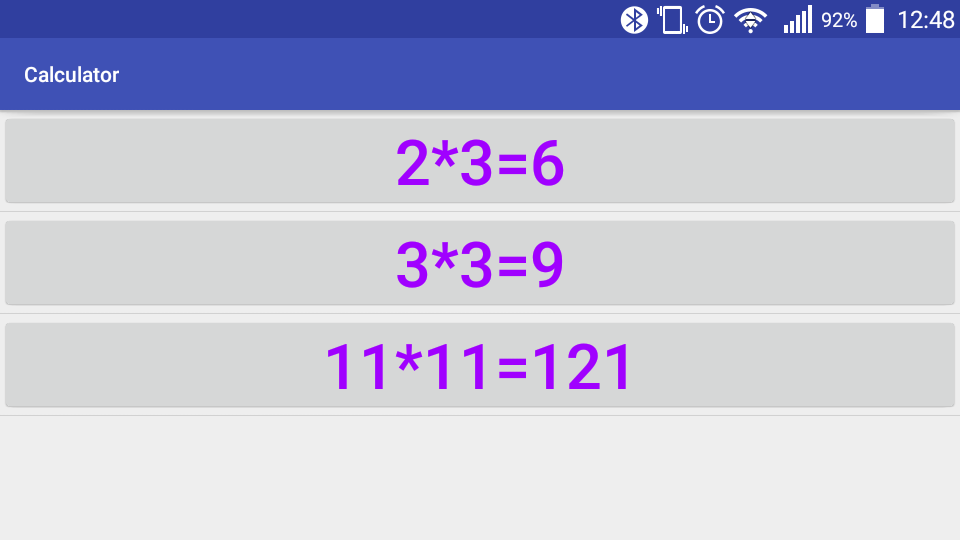
\includegraphics[scale=0.3]{07-list-views/Screenshot.png}

    ListView -- виджет прокручиваемого списка.
    

\Subsection{Adapter, Класс ArrayAdapter, создание списка}\\

    Добавим в XML нужной Activity ListView. 

    \xmlcode{07-list-views/activity_history.xml}
    
    Добавим в onCreate строчки:
    
    \javacode{07-list-views/onCreate.java}

    Заполненный ListView появится на экране.
    
    Для заполнения ListView используется адаптер. 
    
    В этом пример используется ArrayAdapter<>.
    
    Праметры конструктора ArrayAdapter<>:
    \begin{itemize}
        \item this -- контекст
        \item R.layout.my$\_$super$\_$list$\_$item -- собственная разметка для элемента ListView.
        \item вместо history может быть массив объектов с методом toString();
    \end{itemize}

\Subsection{Создание списка из макета (.xml)}
    
    String [] можно получать из xml.
    
    \javacode{07-list-views/default_history.xml}
    
    Код заполнения почти не изменился:
    
    \javacode{07-list-views/onCreate2.java}